\documentclass[crop=false]{standalone}

\usepackage[subpreambles=false]{standalone}
\usepackage{import}
\usepackage{graphicx}
\usepackage{subcaption}
\usepackage{tikz}

\begin{document}

\begin{figure*}
  \centering
  % \hspace*{-0.08\linewidth}
  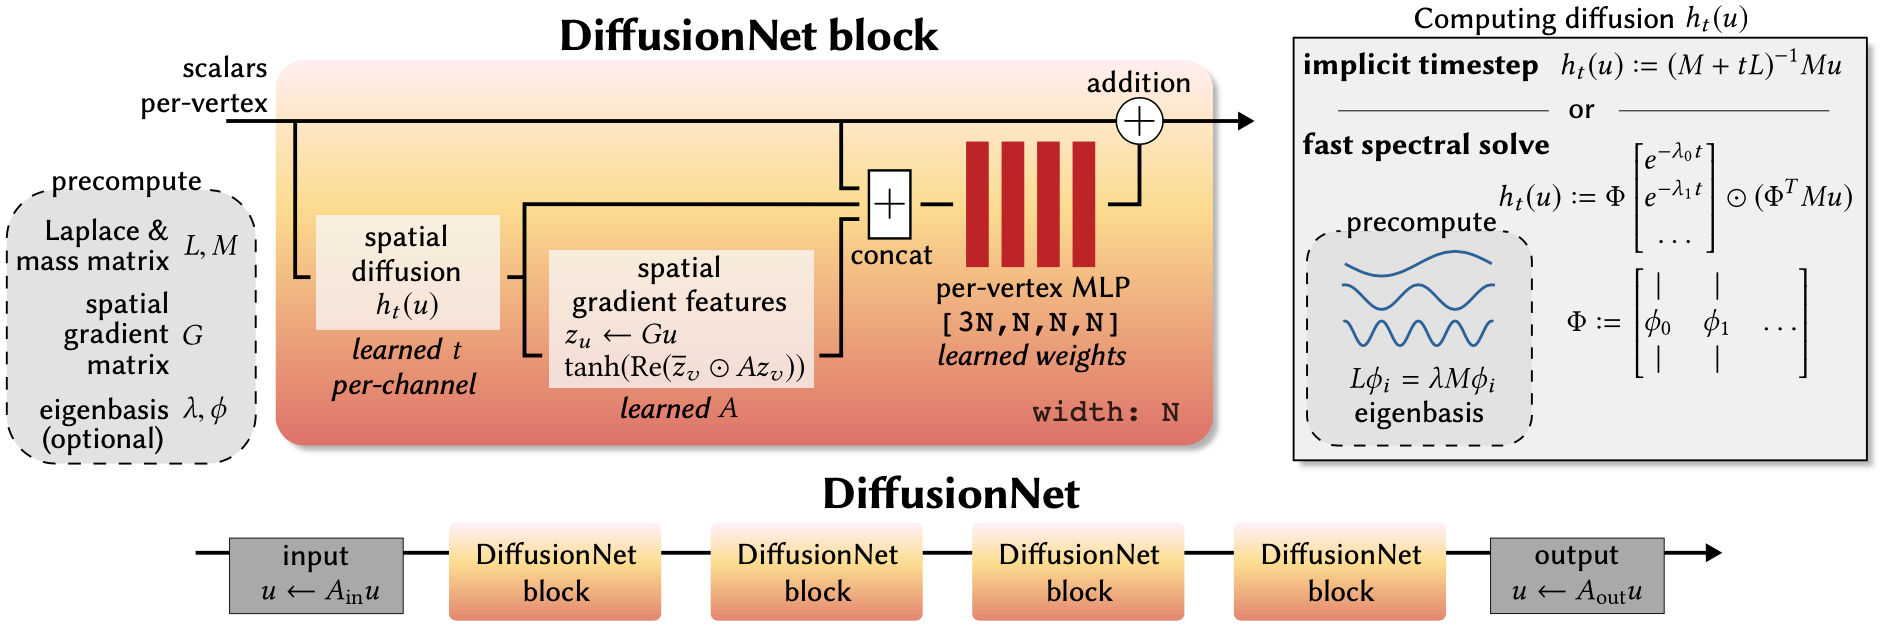
\includegraphics[width=\linewidth]{thesis/methods/import/imgs/diffusionnet_architecture.png}
  %\vspace*{-0.06\linewidth}
  \captionof{figure}{
    \textbf{DiffusionNet architecture.}
    \small After the precomputation of necessary operators, the input is applied to several blocks. In each block, spatial gradients and diffused features are fed into a point-wise MLP with shared weights, and residual connections facilitate training. In this work, diffusion is computed by spectral acceleration. Taken from \cite{sharp2022diffusion}.
  }
  \label{fig:diffusionnet_architecture}
\end{figure*}

\end{document}